\chapter{Design Front-End}
\thispagestyle{stdPage}

%capo la mia conoscienza di latex si sta espandendo però probabilmente questo non compila comunque, halp me plz
% ho fatto del mio meglio per preparare un brodo degno di gordon ramsay

\section{Pagina Iniziale}

    \begin{figure}[H]
        \center
        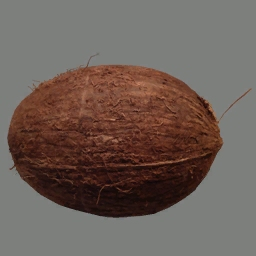
\includegraphics[width=0.33\textwidth]{placeholder.jpg} %PLACEHOLDER QUI CI VA LA PRIMA SLIDE DI LUCA
        \caption{Figura 1 PLACEHOLDER}
    \end{figure}

    La Figura 1 mostra un mockup della principale dell'applicazione, questa schermata sarà visibile a tutti gli utenti.

    \begin{itemize} %sono piuttosto sicuro che questa lista uscira tutta incasinata
        \item RF1: La homepage dell'applicazione mostra la mappa del Comune di Trento in primo piano, sono visibili anche i confini tra i singoli quartieri della città
        \item RF2: L'interfaccia contiene tre pulsanti, ognuno contenente una bandiera corrispondente a una delle lingue supportate dall'applicazione (italiano, inglese, tedesco). Cliccare sui pulsanti cambierà la lingua in cui è presentata l'interfaccia grafica 
        \item RF5: L'interfaccia presenta un pulsante, rappresentato da un'icona, che permette di iniziare il processo di autenticazione degli utenti. Questo permette agli utenti loggati di acceder al proprio account tramite SPID, CNS, CIE, CPS; come dettato dal requisito.
        \item RNF9: La grafica disponibile a tutti gli utenti utilizza un design chiaro, usando icone per rendere la navigazione dell'interfaccia il più accessibile possibile
        \item RNF11: All'inizio, l'interfaccia sarà presentata in lingua italiana. Il design include pulsanti, sempre presenti nella parte alta della schermata, per cambiare la lingua in inglese o tedesco
    \end{itemize}



\section{Utente Loggato, Dati in Tabella}

    \begin{figure}[H]
        \center
        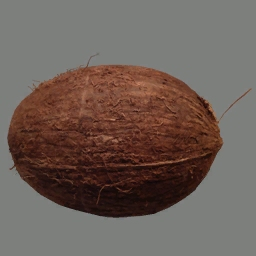
\includegraphics[width=0.33\textwidth]{placeholder.jpg} %PLACEHOLDER QUI CI VA LA SECONDA SLIDE DI LUCA
        \caption{Figura 2 PLACEHOLDER}
    \end{figure}    

    La Figura 2 mostra il mockup della schermata visibile a qualsiasi utente loggato una volta eseguito l'accesso al proprio account

    \begin{itemize}
        \item RF5: Dopo essere stata eseguita l'autenticazione, l'icona di login è sostituita dall'immagine di profilo dell'utente. Inoltre è presente il pulsante per aprire il menù a tendina per permettere all'utente di usufruire delle funzionalità abilitate al proprio account e di eseguire il logout
        \item RF6: Sebbene il mockup mostri i dati dell'applicazione in una tabella, questa funzionalità sarà attiva solo quando l'utente loggato possiede un account analista. Gli altri tipi di utenti loggati vedranno i dati sulla mappa come nella Figura 1.
    \end{itemize}




\section{Selezione di un Quartiere}

    \begin{figure}[H]
        \center
        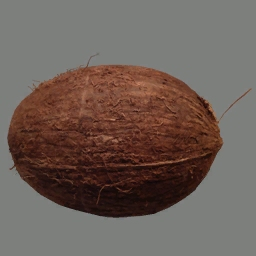
\includegraphics[width=0.33\textwidth]{placeholder.jpg} %PLACEHOLDER QUI CI VA LA TERZA SLIDE DI LUCA
        \caption{Figura 3 PLACEHOLDER}
    \end{figure}    

    La Figura 3 mostra il mockup della schermata visibile dopo che l'utente ha cliccato su uno dei quartieri

    \begin{itemize}
        \item RF3: Selezionare un quartiere è possibile cliccandolo sulla mappa. Una volta che un quartiere è selezionato la mappa lo mostra al centro e ingrandito, e le informazioni relative a esso vengono presentate al fianco della mappa. Nel mockup l'interfaccia mostra solo i dati generali, visibili dagli utenti non loggati. Ma agli account abilitati è consentito osservare anche i dati più approfonditi.
    \end{itemize}


